\section{Kết quả}

Sau quá trình thu thập và tiền xử lý dữ liệu, nghiên cứu đã thu được tổng cộng thông tin của 492 ấn phẩm bị thu hồi được xuất bản từ năm 2021 - 2026. Bảng \tableref{table:retraction_characteristics} trình bày chi tiết các số liệu thống kê tổng quan về tập dữ liệu bao gồm 56 tạp chí đại diện cho 13 nhà xuất bản, quy tụ 1135 tác giả riêng biệt đến từ 42 quốc gia cơ quan công tác khác nhau. Đồng thời, các trường hợp thu hồi được phân loại vào 12 danh mục với tổng số 35 nhãn lý do chi tiết.

\begin{table}[H]
\caption{Đặc điểm xuất bản và nghiên cứu của các bài báo bị thu hồi.}
\label{table:retraction_characteristics}
\begin{tabular*}{\textwidth}{@{} l @{\extracolsep{\fill}} r @{}}
\toprule
\textbf{Đặc điểm} & \textit{\textbf{n}} $\textbf{= 501}$ \\
\midrule
\textit{\textbf{Đặc điểm xuất bản}} & \\
Số lượng các tạp chí học thuật quốc tế có ấn phẩm bị thu hồi & 60 \\
Khoảng thời gian xuất bản của các bài báo trong tập dữ liệu & 2021 - 07/2026 \\
Tổng số các nhà xuất bản học thuật quản lý các tạp chí liên quan & 15 \\
\addlinespace
\textit{\textbf{Tác giả và địa lý}} & \\
Số lượng tác giả (được định danh theo mã ID duy nhất trên hệ thống) & 1155 \\
Số lượng các quốc gia có cơ quan hoặc đơn vị công tác của tác giả & 44 \\
\addlinespace
\textit{\textbf{Lý do thu hồi}} & \\
Tổng số danh mục phân loại lý do thu hồi chính & 12 \\
Số lượng các nhãn chi tiết cụ thể mô tả lý do thu hồi bài báo & 35 \\
\bottomrule
\end{tabular*}
\end{table}

{\noindent\robotocondensed\footnotesize Dữ liệu được trình bày dưới dạng tổng số lượng.}

\subsection{Số lượng ấn phẩm và thời gian thu hồi theo thời gian}

Số lượng ấn phẩm bị thu hồi (Hình \figref{fig:volume-chart}) tăng mạnh từ 7 bài năm 2021 lên 81 bài năm 2022, đạt đỉnh 307 bài vào năm 2023, sau đó giảm đáng kể xuống 60 bài năm 2024 và 26 bài năm 2025. Đến tháng 7/2026, dữ liệu ghi nhận 12 bài, tương ứng mức giảm 96,09\% so với đỉnh năm 2023. Diễn biến này cho thấy số lượng ấn phẩm bị thu hồi không tăng theo một xu hướng liên tục mà có tính đột biến theo thời điểm, trong đó năm 2023 nổi bật như một sự kiện thu hồi quy mô lớn, sau đó hoạt động thu hồi nhanh chóng trở về mức thấp hơn. Mô hình này cho thấy sự gia tăng trong năm 2023 có khả năng phản ánh một đợt thu hồi hàng loạt do nhà xuất bản dẫn dắt, thay vì sự gia tăng bền vững của hoạt động thu hồi.

\begin{figure}[H]
    \centering
    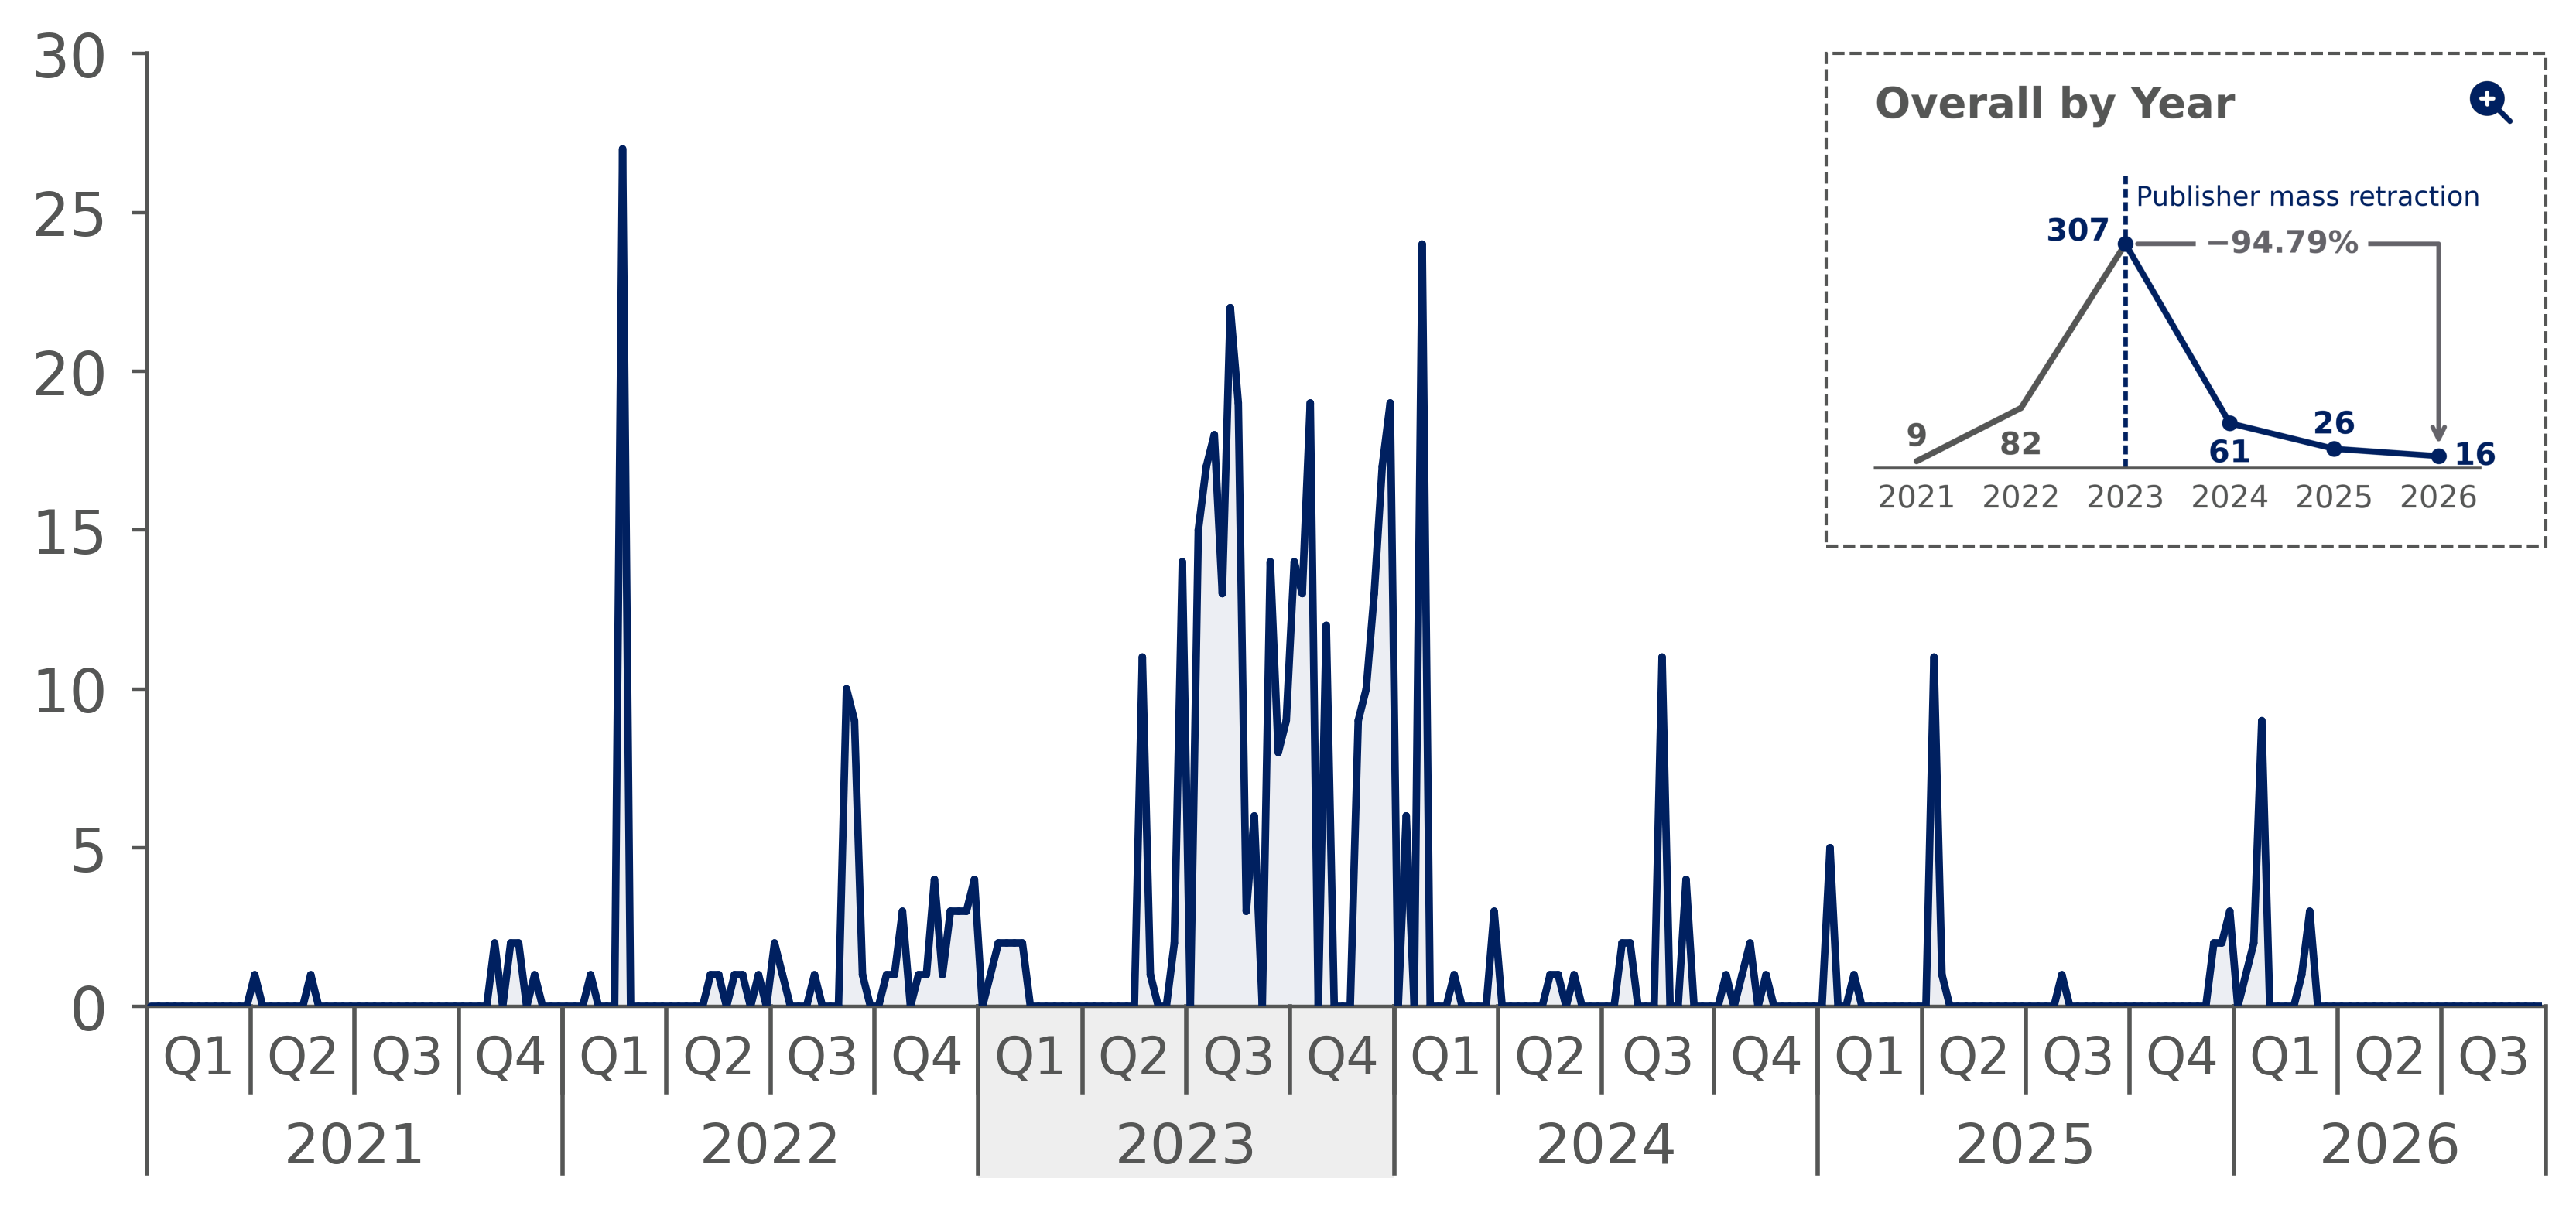
\includegraphics[width=\textwidth, left]{figures/results/volume-chart.png}
    \caption{Xu hướng số lượng ấn phẩm ngành Khoa học Thông tin và Thư viện bị thu hồi qua từng năm giai đoạn 2021 - 2026}
    \label{fig:volume-chart}
\end{figure}

\begin{figure}[H]
    \centering
    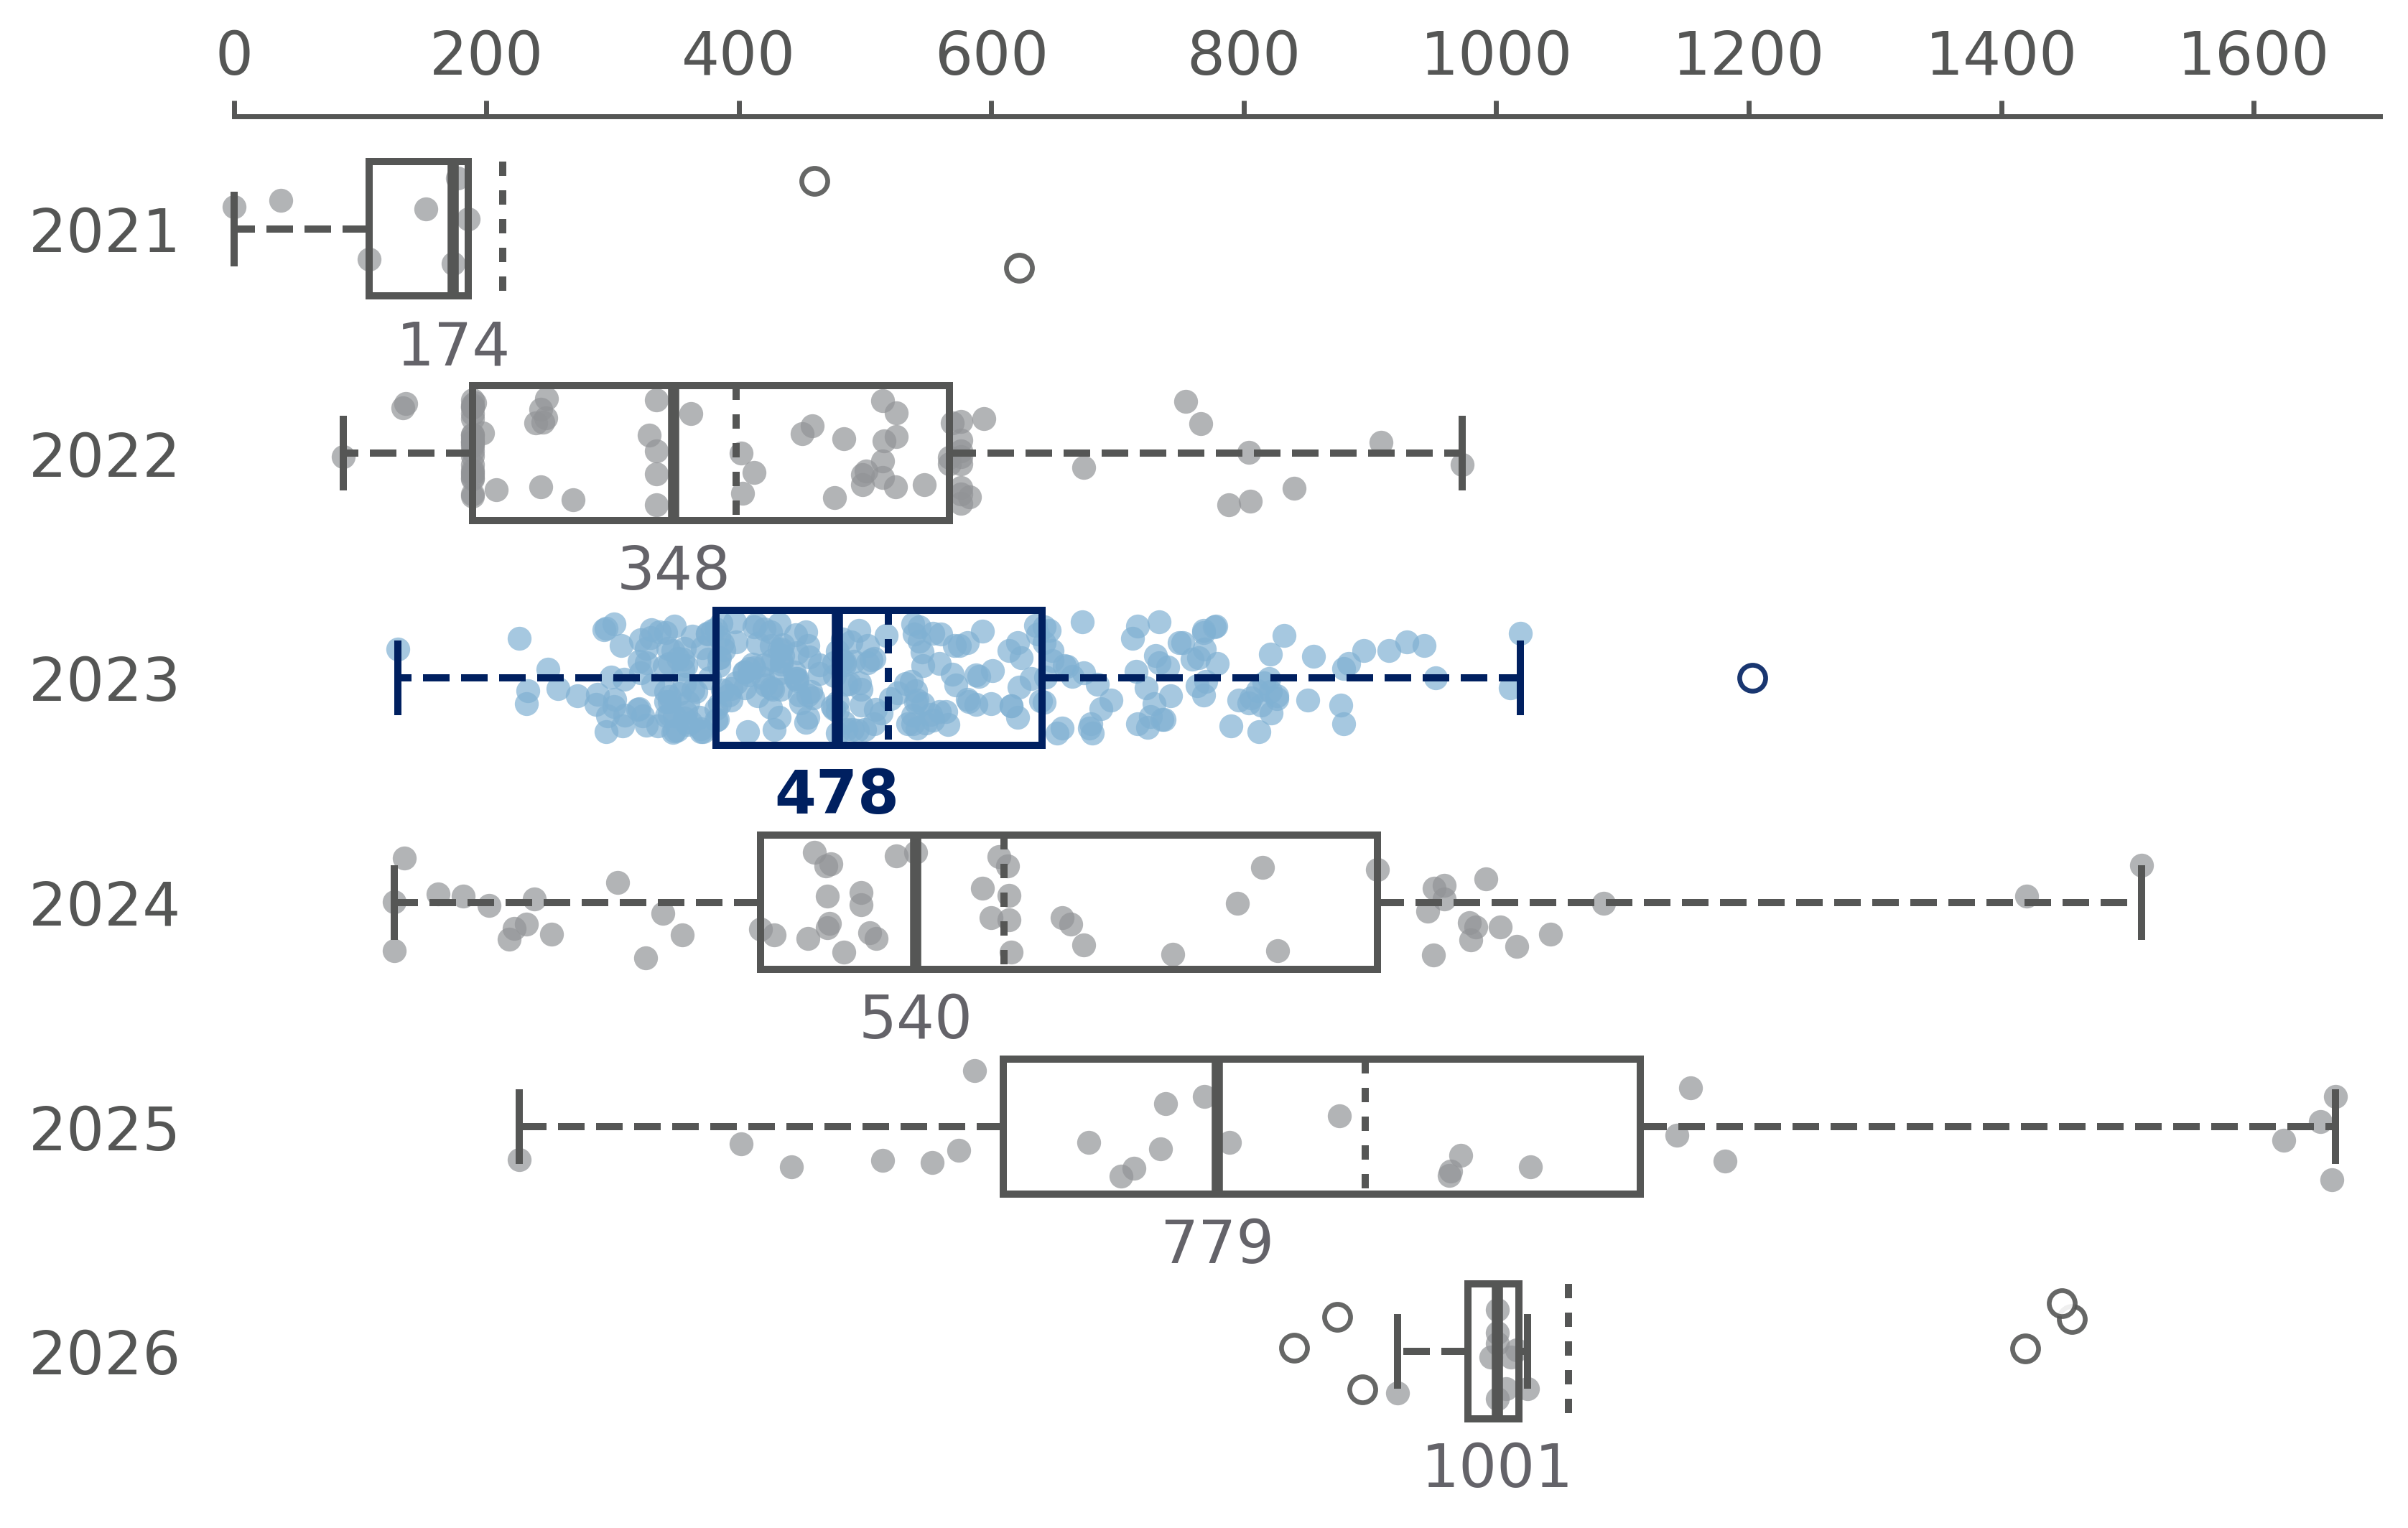
\includegraphics[width=\textwidth]{figures/results/lag-days-chart.png}
    \caption{Phân phối thời gian thu hồi ấn phẩm ngành Khoa học Thông tin và Thư viện bị thu hồi qua từng năm giai đoạn 2021 - 2026}
    \label{fig:lag-days-chart}
\end{figure}

Độ trễ từ thời điểm công bố đến khi thu hồi có xu hướng tăng dần qua các năm. Trung vị độ trễ tăng từ khoảng 150 ngày năm 2021 lên 330 ngày năm 2022, 480 ngày năm 2023, 570 ngày năm 2024 và khoảng 780 ngày năm 2025. Các quan sát của năm 2026 cho thấy trung vị tiếp tục ở mức cao, khoảng 1.000 ngày, tuy nhiên kết quả này cần được diễn giải thận trọng do dữ liệu năm 2026 mới chỉ được ghi nhận đến tháng 7. Bên cạnh sự gia tăng của trung vị, phân phối từ năm 2023 trở đi cũng cho thấy mức độ phân tán lớn hơn, với nhiều trường hợp có độ trễ trên 1.000 ngày và một số giá trị cực trị vượt 1.500 ngày. Điều này cho thấy thời gian từ khi công bố đến khi bị thu hồi có sự khác biệt đáng kể giữa các ấn phẩm và có xu hướng kéo dài ở những năm gần đây.

Đáng chú ý, năm 2023 có số lượng ấn phẩm bị thu hồi cao nhất nhưng không có độ trễ thu hồi cao nhất. Mặc dù số lượng thu hồi tăng đột biến trong năm này, thời gian trung vị từ khi công bố đến khi thu hồi vẫn thấp hơn so với các năm 2024 - 2026. Điều này cho thấy số lượng ấn phẩm bị thu hồi và thời gian để một ấn phẩm bị thu hồi không nhất thiết biến động theo cùng một xu hướng. Nói cách khác, đợt thu hồi hàng loạt trong năm 2023 không đồng nghĩa với việc các ấn phẩm trong đợt này phải mất nhiều thời gian hơn mới được phát hiện và thu hồi.

\begin{figure}[H]
    \centering
    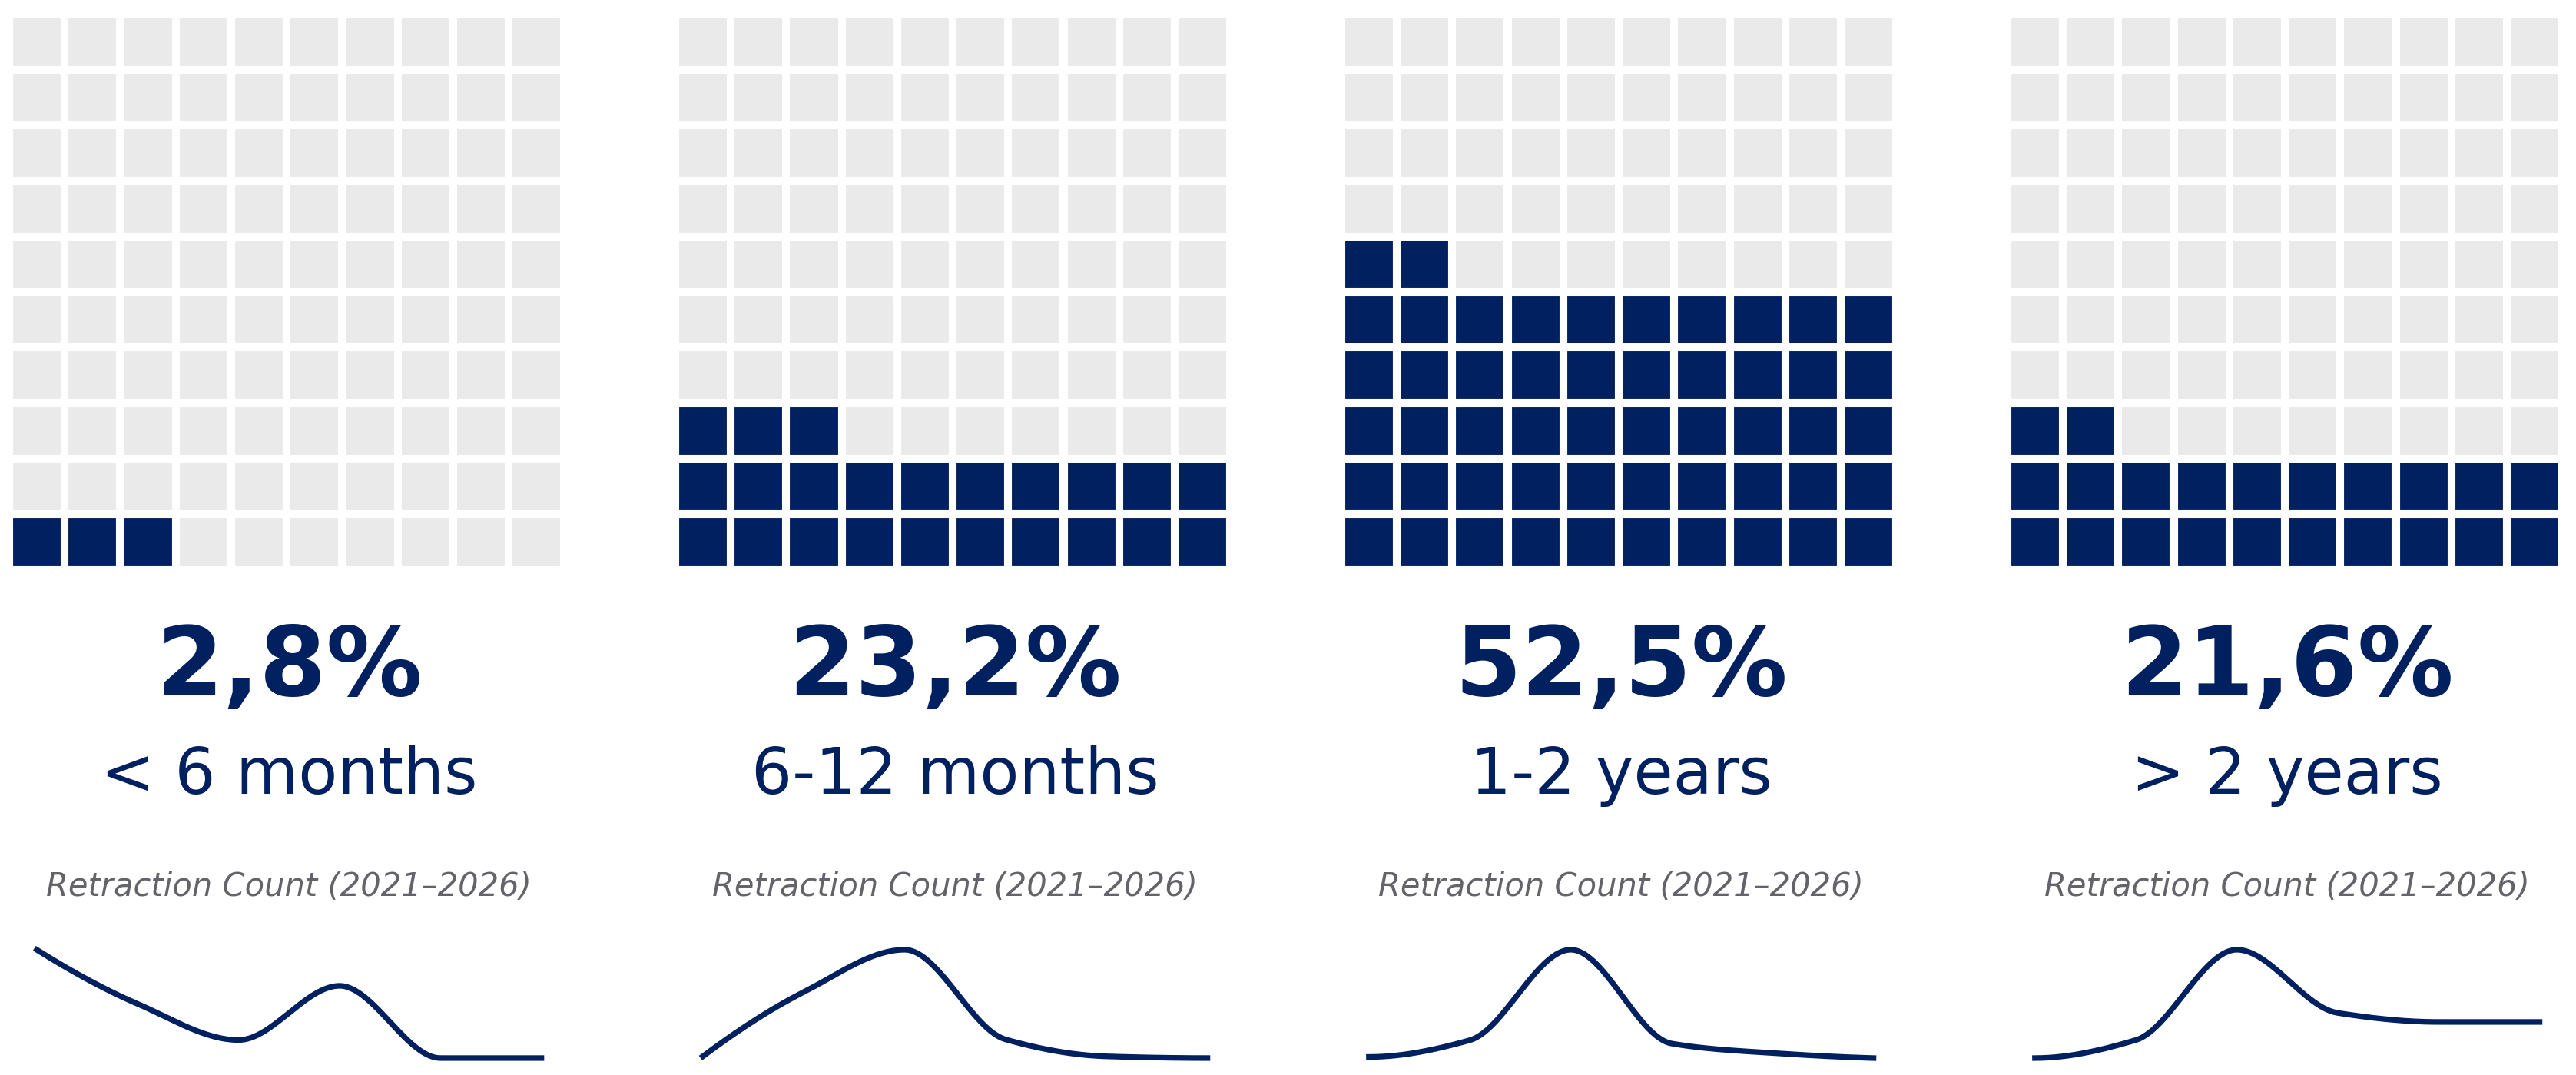
\includegraphics[width=\textwidth]{figures/results/retraction-lag-day-square-chart.png}
    \caption{Phân bổ và xu hướng thu hồi tài liệu theo các nhóm thời gian trễ từ khi xuất bản (< 6 tháng, 6-12 tháng, 1-2 năm, > 2 năm, 2021–2026)}
    \label{fig:retraction-lag-day-square-chart}
\end{figure}

Biểu đồ ở Hình \figref{fig:retraction-lag-day-square-chart} cung cấp góc nhìn toàn diện về khoảng thời gian từ lúc tài liệu ra mắt đến khi chính thức bị thu hồi trong giai đoạn 2021–2026. Trong đó, các trường hợp thu hồi rất sớm dưới 6 tháng chỉ chiếm tỷ lệ vỏn vẹn 2,8\% do độ trễ tự nhiên trong quá trình kiểm duyệt ban đầu, trước khi tăng lên 23,2\% ở nhóm từ 6 đến 12 tháng. Tâm điểm của toàn bộ dữ liệu tập trung áp đảo ở khung thời gian 1 - 2 năm với 52,5\%, phản ánh đây là giai đoạn cao điểm bộc lộ vấn đề và chịu sự can thiệp mạnh mẽ nhất, trước khi chuyển dịch nhẹ và duy trì ở mức 21,6\% đối với các tài liệu lưu hành dài hạn trên 2 năm.

\subsection{Mức độ hợp tác của các tác giả}

\begin{table}[H]
\centering
\caption{Thống kê số lượng bài báo và chỉ số hợp tác theo quốc gia}
\label{tab:country_stats}
\begin{tabular*}{\textwidth}{@{\extracolsep{\fill}} clrrrrrr @{}}
\toprule
\textbf{STT} & \textbf{Quốc gia} & \makecell[r]{\textbf{Tổng số bài}\\\textbf{(\%)}} & \makecell[r]{\textbf{Bài}\\\textbf{nội địa}} & \makecell[r]{\textbf{Bài}\\\textbf{quốc tế}} & \textbf{DCI} & \textbf{ICI} & \makecell[r]{\textbf{Tỷ lệ}\\\textbf{DCI/ICI}} \\
\midrule
1 & China & 432 (86.23\%) & 391 & 41 & 120.06 & 38.56 & 3.1136 \\
2 & India & 35 (6.99\%) & 20 & 15 & 75.80 & 174.13 & 0.4353 \\
3 & Saudi Arabia & 11 (2.20\%) & 3 & 8 & 36.18 & 295.49 & 0.1224 \\
4 & South Korea & 10 (2.00\%) & 1 & 9 & 13.26 & 365.66 & 0.0363 \\
5 & Malaysia & 9 (1.80\%) & 3 & 6 & 44.22 & 270.86 & 0.1633 \\
6 & Philippines & 7 (1.40\%) & 3 & 4 & 56.85 & 232.17 & 0.2449 \\
7 & United States & 6 (1.20\%) & 0 & 6 & 0.00 & 406.29 & 0.0000 \\
8 & Macao & 5 (1.00\%) & 1 & 4 & 26.53 & 325.03 & 0.0816 \\
9 & Pakistan & 5 (1.00\%) & 0 & 5 & 0.00 & 406.29 & 0.0000 \\
10 & Ethiopia & 5 (1.00\%) & 0 & 5 & 0.00 & 406.29 & 0.0000 \\
\bottomrule
\end{tabular*}
\end{table}

\begin{figure}[H]
    \centering
    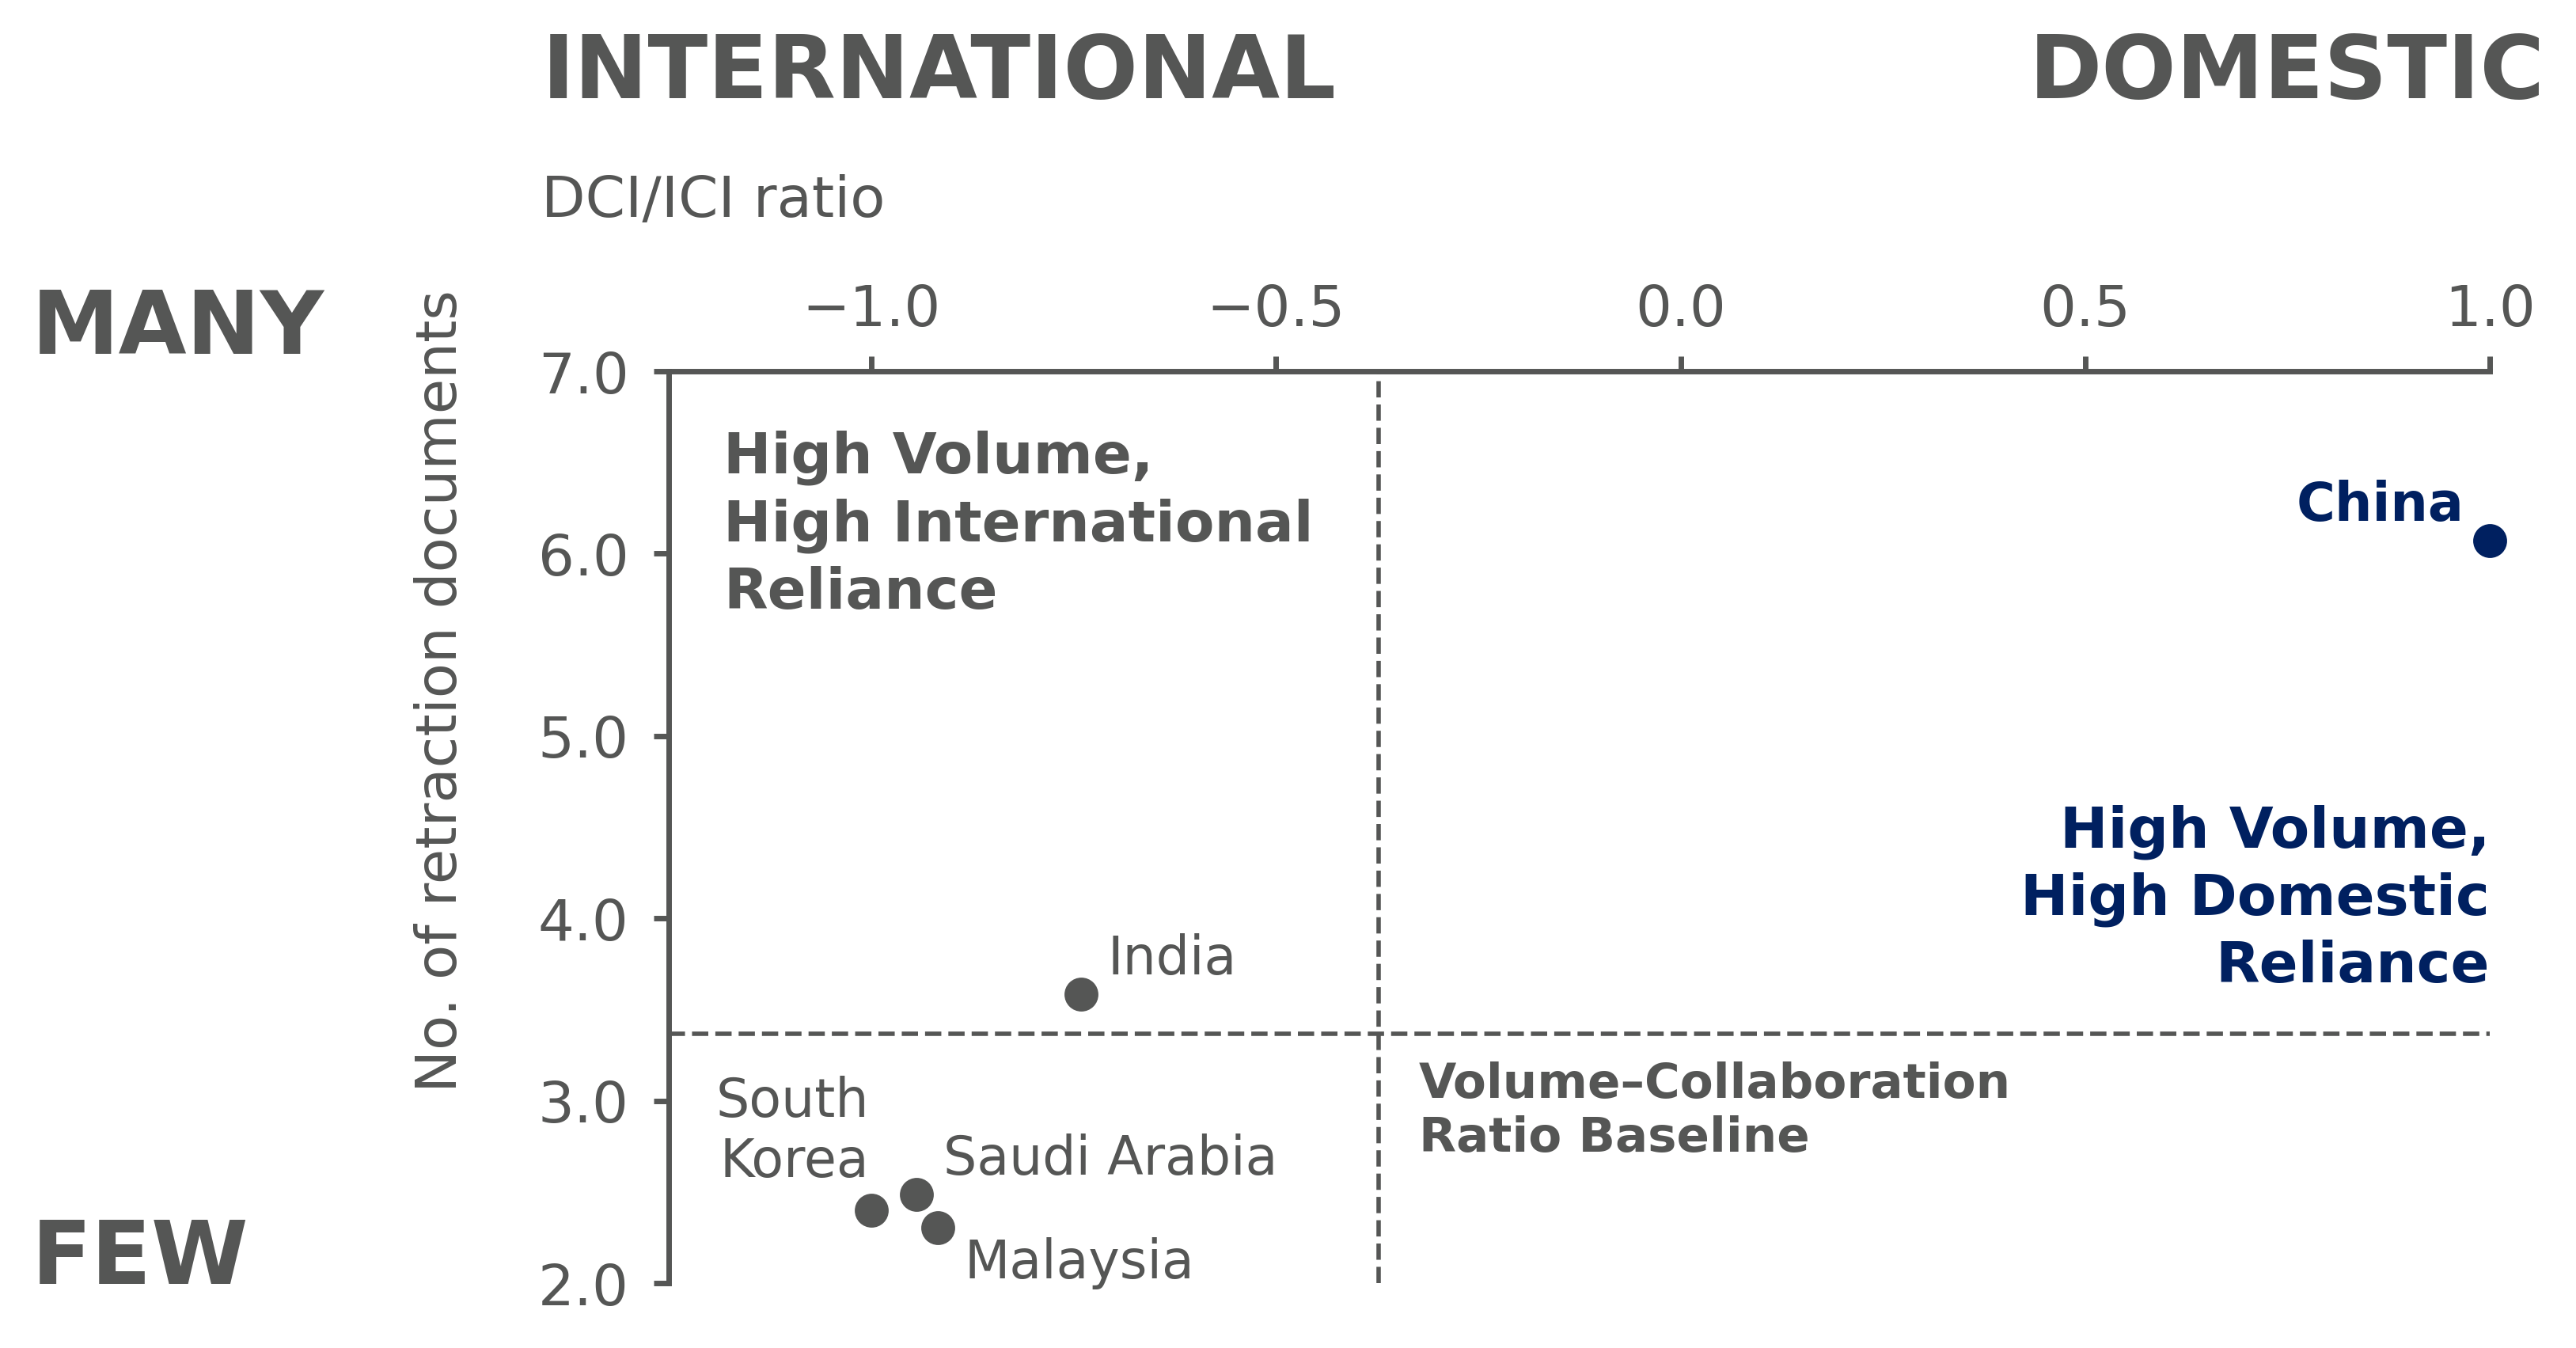
\includegraphics[width=\textwidth]{figures/results/dci-ici-quarter-chart.png}
    \caption{Phân nhóm 5 quốc gia dẫn đầu về khối lượng bài báo và xu hướng hợp tác quốc tế/nội địa}
    \label{fig:dci-ici-quarter-chart}
\end{figure}

Theo Hình \figref{fig:dci-ici-quarter-chart}, để xử lý độ lệch lớn giữa các quốc gia, biểu đồ sử dụng thang đo $\log(N+1)$ ở trục tung nhằm nén dải giá trị bài báo rút lại giúp quan sát rõ các mức từ ít đến rất nhiều mà không bị chênh lệch ảo, kết hợp $\text{Min-Max scaling}$ ở trục hoành để chuẩn hóa tỷ lệ hợp tác về khoảng [-1, 1] cho việc phân chia góc phần tư. Về mặt số liệu, Trung Quốc đạt khối lượng bài rút lại cao vượt trội (trên 6.0 trên thang log) với xu hướng nghiêng về nội địa (gần 1.0), trong khi nhóm gồm Ấn Độ, Hàn Quốc, Ả Rập Xê Út và Malaysia có khối lượng thấp hơn (2.0 - 4.0) và thiên về hợp tác quốc tế. Pattern này phản ánh sự phân hóa rõ rệt giữa quy mô xuất bản lớn gắn với hợp tác nội địa và quy mô nhỏ gắn với hợp tác quốc tế, qua đó khách quan hóa đặc thù phân bố dữ liệu học thuật của từng nhóm quốc gia mà không mang hàm ý đánh giá chất lượng hay quy kết nguyên nhân.

\begin{figure}[H]
    \centering
    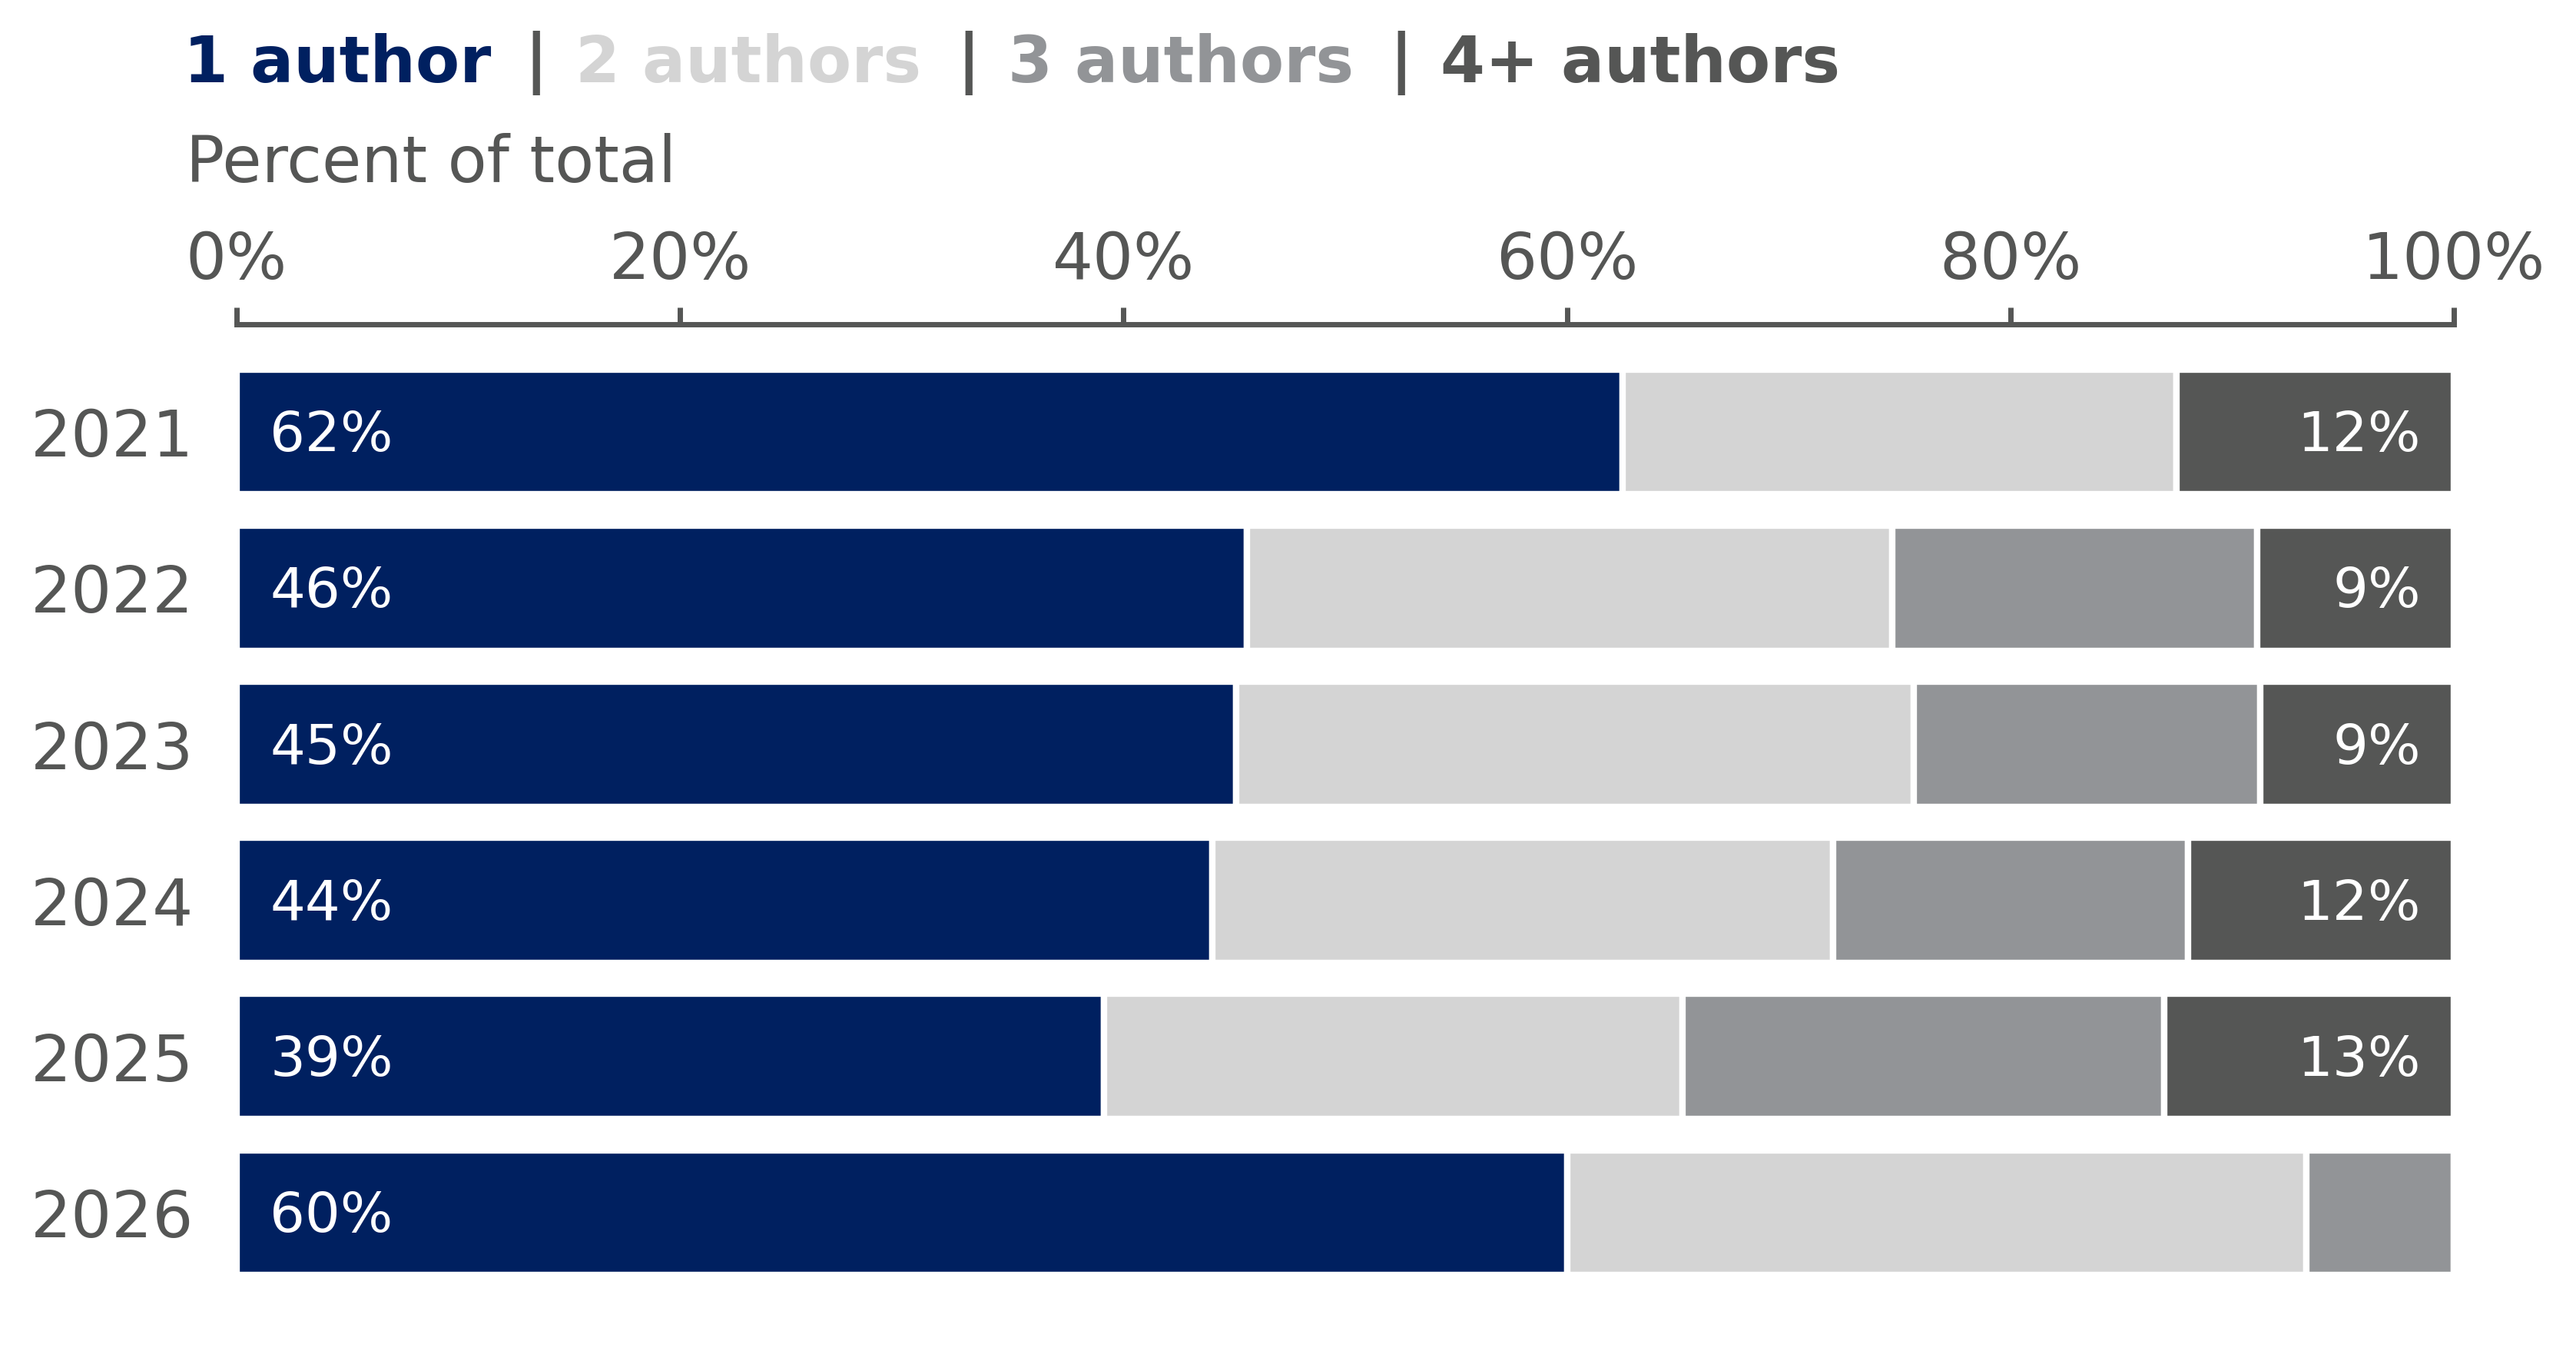
\includegraphics[width=\textwidth, left]{figures/results/authorship-chart.png}
    \caption{Xu hướng số lượng tác giả đứng tên trên mỗi ấn phẩm theo năm}
    \label{fig:authorship-chart}
\end{figure}


\subsection{Đặc điểm phân bố theo lĩnh vực, tạp chí và nhà xuất bản}

\begin{figure}[H]
    \centering
    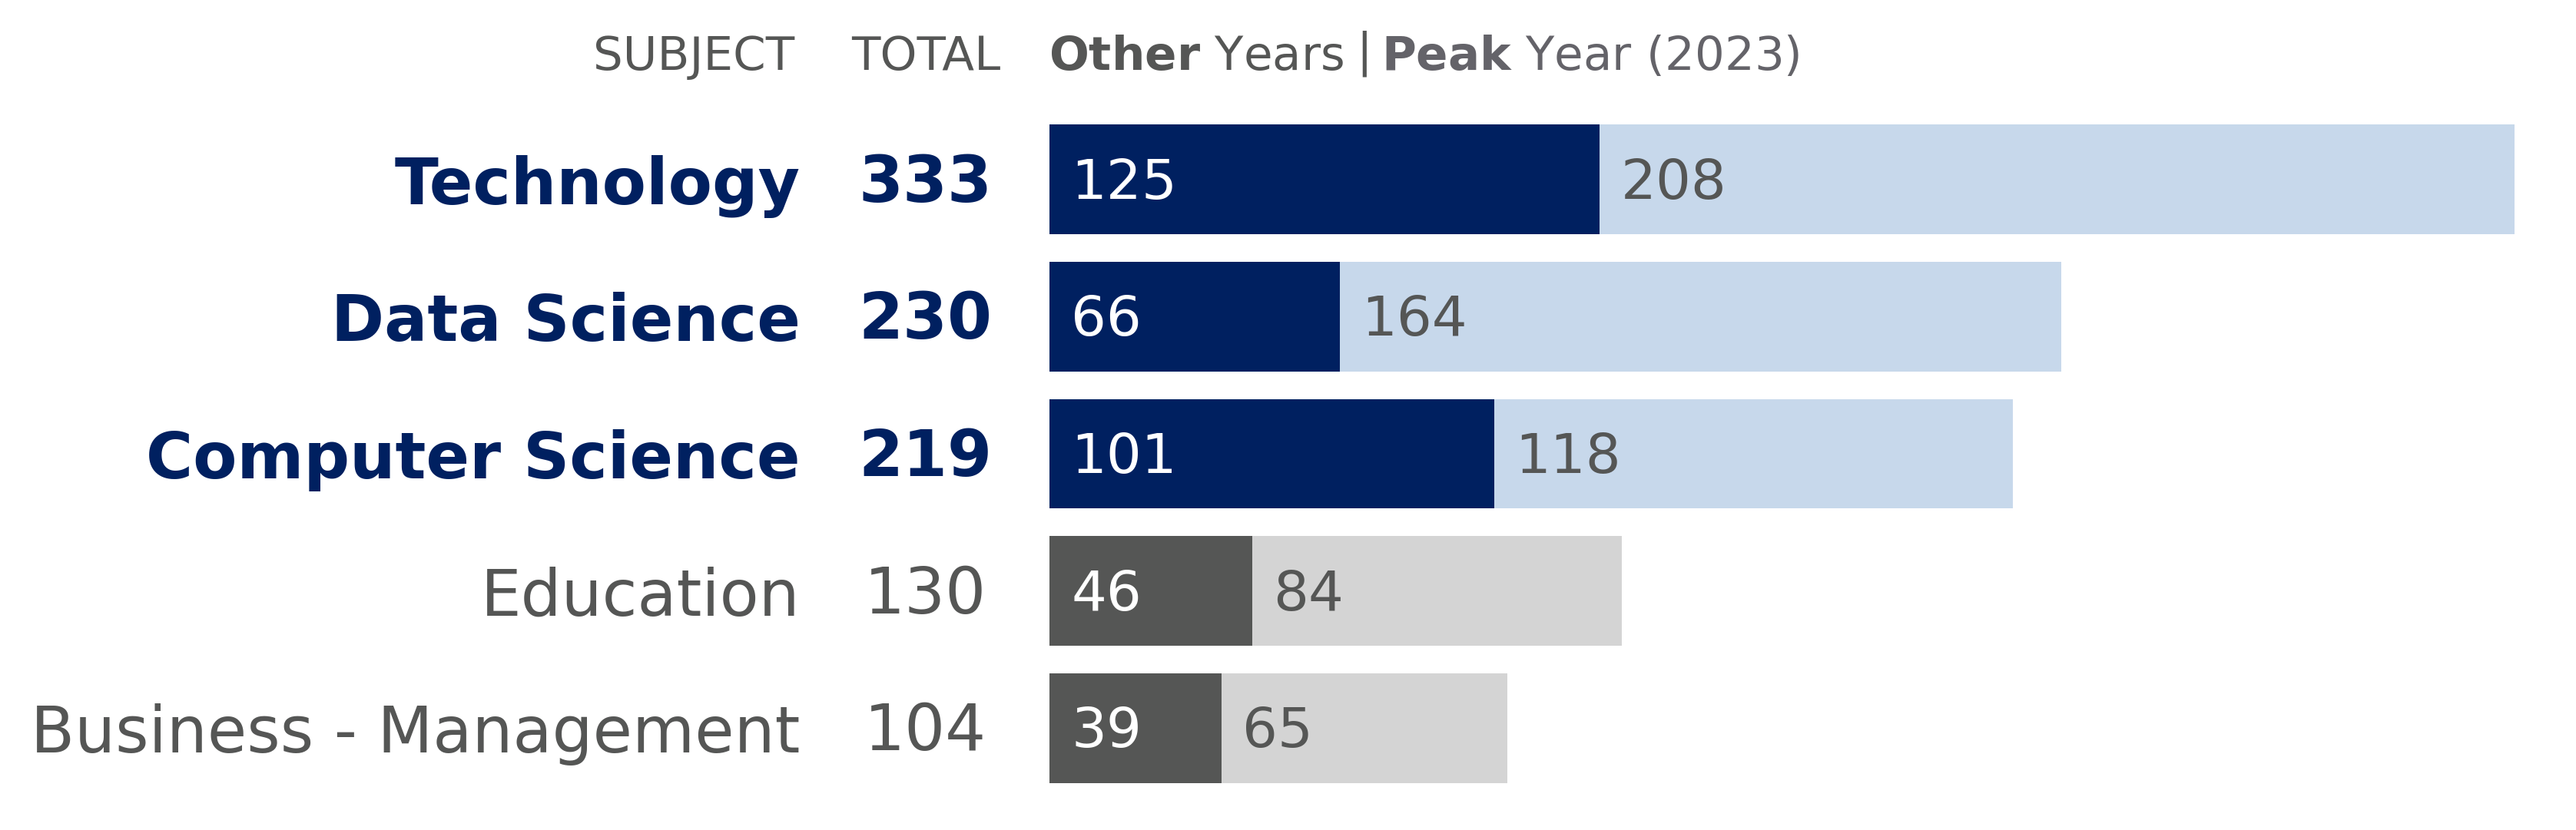
\includegraphics[width=\textwidth]{figures/results/retraction-subject-chart.png}
    \caption{Phân nhóm 5 quốc gia dẫn đầu về khối lượng bài báo và xu hướng hợp tác quốc tế/nội địa}
    \label{fig:retraction-subject-chart}
\end{figure}

Theo Hình \figref{fig:retraction-subject-chart}, các số liệu chi tiết ghi nhận lĩnh vực Technology đạt 333 trường hợp thu hồi, Data Science đạt 230 trường hợp, Computer Science đạt 219 trường hợp, Education đạt 130 trường hợp và Business - Management đạt 104 trường hợp, với nhóm gộp (B/T): Business and Technology (bao gồm Business - Management, Data Science và Technology) đạt tổng cộng 667 trường hợp; qua đó phản ánh mẫu hình chung (pattern) là sự phân hóa rõ rệt với mức độ tập trung cao của các bài báo bị thu hồi ở các lĩnh vực công nghệ và khoa học dữ liệu so với các nhóm ngành giáo dục và quản lý theo đúng đặc điểm phân bố thực tế của dữ liệu.

\begin{figure}[H]
    \centering
    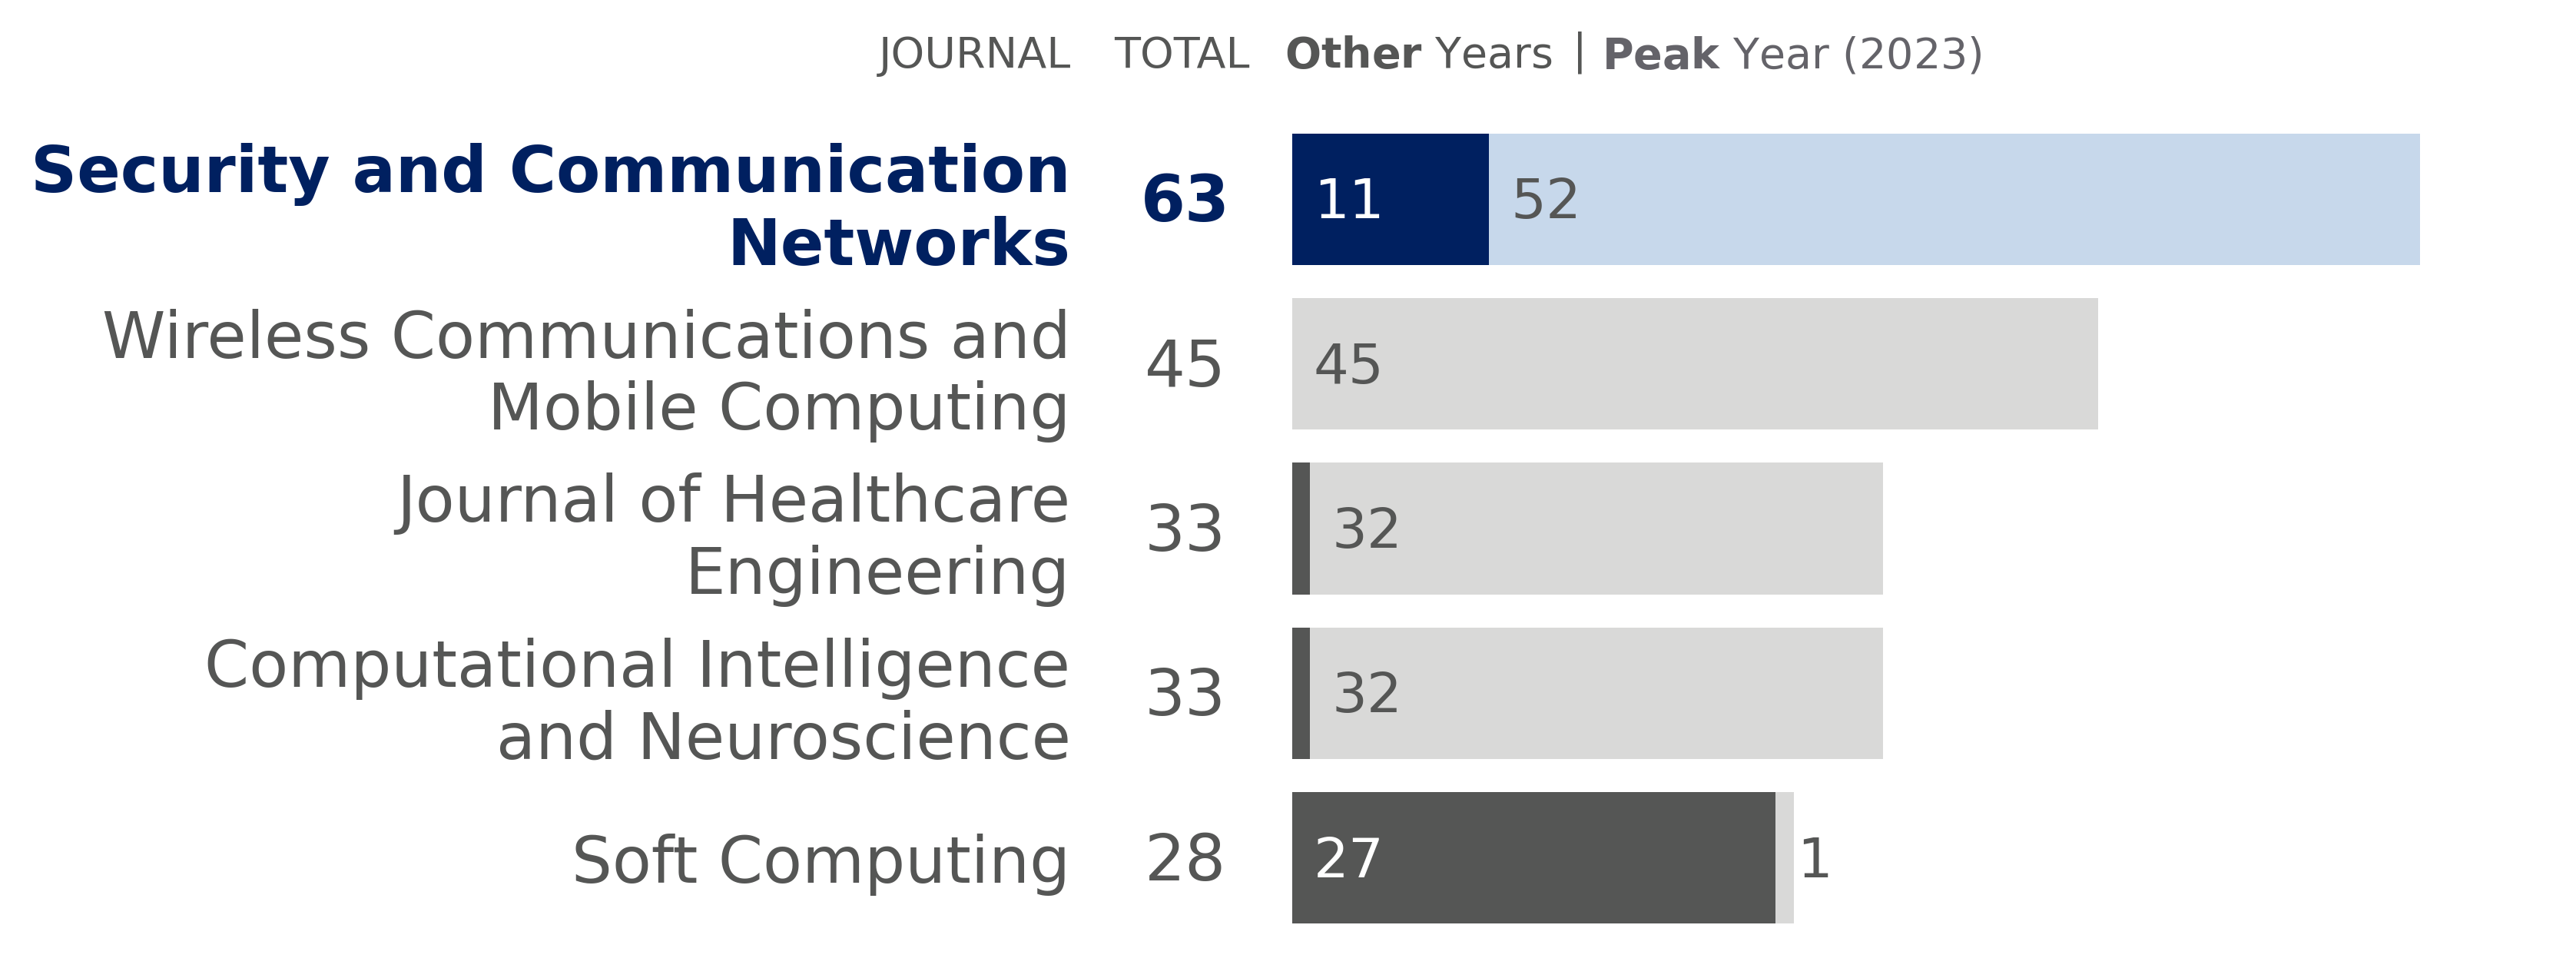
\includegraphics[width=\textwidth]{figures/results/retraction-journal-chart.png}
    \caption{Phân nhóm 5 quốc gia dẫn đầu về khối lượng bài báo và xu hướng hợp tác quốc tế/nội địa}
    \label{fig:retraction-journal-chart}
\end{figure}

Theo Hình \figref{fig:retraction-journal-chart}, bức tranh tổng quan về sự phân bố bài báo bị thu hồi theo các tạp chí cho thấy mức độ tập trung cao tại các ấn phẩm chuyên về mạng và truyền thông, với các giá trị giảm dần theo quy mô của từng tạp chí. Cụ thể, dẫn đầu danh sách là Security and Communication Networks với 63 trường hợp, tiếp nối bởi Wireless Communications and Mobile Computing ở mức 45 trường hợp. Các vị trí tiếp theo ghi nhận sự tương đồng về số lượng giữa Journal of Healthcare Engineering và Computational Intelligence and Neuroscience (cùng đạt 33 trường hợp), trong khi Soft Computing khép lại nhóm với mức 28 trường hợp.

\begin{figure}[H]
    \centering
    
\includegraphics[width=\textwidth]{figures/results/retraction-publisher-chart.png}
    \caption{Phân nhóm 5 quốc gia dẫn đầu về khối lượng bài báo và xu hướng hợp tác quốc tế/nội địa}
    \label{fig:retraction-publisher-chart}
\end{figure}

Theo Hình \figref{fig:retraction-publisher-chart}, bức tranh phân bố số lượng bài báo bị thu hồi theo nhà xuất bản cho thấy sự chênh lệch áp đảo từ một đơn vị duy nhất so với phần còn lại. Cụ thể, Hindawi dẫn đầu với mức vượt trội lên đến 345 trường hợp thu hồi. Ở khoảng cách thấp hơn đáng kể, Springer - Nature Publishing Group ghi nhận 39 trường hợp, tiếp nối bởi IOS Press (bought by Sage November 2023) với 25 trường hợp, trong khi hai vị trí khép lại nhóm là Association for Computing Machinery (ACM) và Springer với cùng 23 trường hợp.

\subsection{Sự khác biệt về khối lượng trong nguyên nhân thu hồi}

{\fontsize{11pt}{12pt}\selectfont
\begin{longtable}{
    >{\raggedright\arraybackslash}p{0.17\textwidth}
    >{\raggedright\arraybackslash}p{0.45\textwidth}
    >{\raggedleft\arraybackslash}p{0.14\textwidth}
    >{\raggedleft\arraybackslash}p{0.14\textwidth}
}
\caption{Tổng hợp chi tiết và tổng số lý do thu hồi ấn phẩm theo danh mục}
\label{table:merged_retraction_reasons} \\
\toprule
\textbf{Retraction Category} &
\textbf{Retraction Subcategory} &
\textbf{No. (\%)} &
\textbf{Total, No. (\%)} \\
\midrule
\endfirsthead

\caption[]{\textit{(Tiếp theo)} Tổng hợp chi tiết và tổng số lý do thu hồi ấn phẩm theo danh mục} \\
\toprule
\textbf{Retraction Category} &
\textbf{Retraction Subcategory} &
\textbf{No. (\%)} &
\textbf{Total, No. (\%)} \\
\midrule
\endhead

% Legal Issues
\multirow[t]{10}{=}{Legal Issues}
& Investigation by Journal/Publisher
& 487 (14,65 \%)
& \multirow[t]{10}{=}{948 (28,45 \%)} \\
& Investigation by Third Party
& 343 (10,32 \%)
& \\
& Rogue Editor
& 54 (1,62 \%)
& \\
& Author Unresponsive
& 18 (0,54 \%)
& \\
& Objections by Author(s)
& 18 (0,54 \%)
& \\
& Concerns/Issues about Third Party Involvement
& 21 (0,63 \%)
& \\
& Removed
& 4 (0,12 \%)
& \\
& Investigation by Company/Institution
& 1 (0,03 \%)
& \\
& Objections by Third Party
& 1 (0,03 \%)
& \\
& Temporary Removal
& 1 (0,03 \%)
& \\
\midrule

% Data Concerns
\multirow[t]{7}{=}{Data Concerns}
& Unreliable Results and/or Conclusions
& 397 (11,94 \%)
& \multirow[t]{7}{=}{915 (27,49 \%)} \\
& Concerns/Issues about Data
& 276 (8,30 \%)
& \\
& Concerns/Issues about Results and/or Conclusions
& 237 (7,13 \%)
& \\
& Unreliable Data
& 2 (0,06 \%)
& \\
& Error in Data
& 1 (0,03 \%)
& \\
& Unreliable Image
& 1 (0,03 \%)
& \\
& Original Data and/or Images not Provided
& 1 (0,03 \%)
& \\
\midrule

% Peer Review Issues
\multirow[t]{2}{=}{Peer Review Issues}
& Concerns/Issues about Peer Review
& 312 (9,38 \%)
& \multirow[t]{2}{=}{500 (15,03 \%)} \\
& Compromised Peer Review
& 188 (5,65 \%)
& \\
\midrule

% Referencing Issues
Referencing Issues
& Concerns/Issues about Referencing/Attributions
& 335 (10,08 \%)
& 335 (10,06 \%) \\
\midrule

% Fraud
\multirow[t]{2}{=}{Fraud}
& Paper Mill
& 260 (7,82 \%)
& \multirow[t]{2}{=}{\raggedleft 261 (7,83 \%)} \\
& False/Forged Authorship
& 1 (0,03 \%)
& \\
\midrule

% Randomly Generated Content
Randomly Generated Content
& Computer-Aided Content or Computer-Generated Content
& 251 (7,55 \%)
& 251 (7,53 \%) \\
\midrule

% Ethical Issues
\multirow[t]{6}{=}{Ethical Issues}
& Lack of IRB/IACUC Approval and/or Compliance
& 39 (1,17 \%)
& \multirow[t]{6}{=}{\raggedleft 78 (2,34 \%)} \\
& Informed/Patient Consent - None/Withdrawn
& 38 (1,14 \%)
& \\
& Concerns/Issues about Human Subject Welfare
& 1 (0,03 \%)
& \\
\midrule

% Authorship Issues
\multirow[t]{2}{=}{Authorship Issues}
& Concerns/Issues about Authorship/Affiliation
& 4 (0,12 \%)
& \multirow[t]{2}{=}{\raggedleft 5 (0,15 \%)} \\
& Taken from Dissertation/Thesis
& 1 (0,03 \%)
& \\
\midrule

% Transparency Issues
\multirow[t]{3}{=}{Transparency Issues}
& Concerns/Issues about Article
& 12 (0,36 \%)
& \multirow[t]{3}{=}{\raggedleft 22 (0,66 \%)} \\
& Upgrade/Update of Prior Notice(s)
& 9 (0,27 \%)
& \\
& Date of Article and/or Notice Unknown
& 1 (0,03 \%)
& \\
\midrule

% Error
Error
& Error by Journal/Publisher
& 1 (0,03 \%)
& 1 (0,03 \%) \\
% Duplication
Duplication
& Duplication of/in Article
& 1 (0,03 \%)
& 1 (0,03 \%) \\
\midrule

% Plagiarism
Plagiarism
& Plagiarism of/in Article
& 1 (0,03 \%)
& 1 (0,03 \%) \\
\midrule

% Others
Others
&
& 
& 1 (0,03 \%) \\

\bottomrule
\end{longtable}
}

Như được trình bày chi tiết trong bảng \tableref{table:merged_retraction_reasons}, bức tranh tổng thể về các nguyên nhân thu hồi ấn phẩm khoa học cho thấy sự phân hóa sâu sắc và tập trung cao độ vào một số nhóm vấn đề cốt lõi thay vì phân bố đồng đều. Dẫn đầu danh sách là hai nhóm \textit{Peer Review Issues} và \textit{Legal Issues} với cùng mức 488 ấn phẩm, chiếm tỷ trọng cao nhất là 20,54\%, trong đó nhóm vấn đề bình duyệt chủ yếu tập trung vào các quan ngại chung về quy trình (312 trường hợp) và tình trạng bình duyệt bị thao túng hoặc xâm phạm (188 trường hợp), còn nhóm pháp lý phần lớn xuất phát từ các cuộc điều tra do tạp chí hoặc nhà xuất bản thực hiện (487 trường hợp) cũng như các cuộc điều tra từ bên thứ ba (343 trường hợp). Xếp ngay sau đó là nhóm \textit{Data Concerns} với 401 ấn phẩm (chiếm 16,88\% N), với trọng tâm là các kết quả hoặc kết luận không đáng tin cậy (397 trường hợp) và các vấn đề liên quan trực tiếp đến dữ liệu (276 trường hợp); tiếp tục theo sau là nhóm \textit{Referencing Issues} ghi nhận 335 ấn phẩm (14,10\%), nhóm \textit{Fraud} chiếm 314 ấn phẩm (13,22\%) nổi cộm bởi hiện tượng xưởng sản xuất bài báo \textit{Paper Mill} (260 trường hợp), và nhóm \textit{Randomly Generated Content} với 251 ấn phẩm (10,56\%). Ngược lại, các nhóm nguyên nhân liên quan đến đạo đức, tác giả và tính minh bạch chiếm tỷ trọng thấp hơn đáng kể trong tổng thể dữ liệu, bao gồm \textit{Ethical Issues} (39 ấn phẩm, 1,64\%), \textit{Authorship Issues} (23 ấn phẩm, 0,97\%), \textit{Transparency Issues} (19 ấn phẩm, 0,80\%), và \textit{Others} (14 ấn phẩm, 0,59\%). Cuối cùng, các nhóm chiếm tỷ lệ tối thiểu trong toàn bộ bảng thống kê là \textit{Error} (2 ấn phẩm, 0,08\%), \textit{Duplication} (1 ấn phẩm, 0,04\%) và \textit{Plagiarism} (1 ấn phẩm, 0,04\%), qua đó phản ánh rõ nét rằng xu hướng thu hồi bài báo hiện nay chủ yếu bắt nguồn từ các sự cố hệ thống, sai sót dữ liệu và các hành vi gian lận tinh vi thay vì các lỗi vi phạm truyền thống như đạo văn hay sao chép thông thường.